%%%%%%%%%%%%%%%%%%%%%%%%%%%%%%%%%%%%%%%%%
% University/School Laboratory Report
% LaTeX Template
% Version 3.1 (25/3/14)
%
% This template has been downloaded from:
% http://www.LaTeXTemplates.com
%
% Original author:
% Linux and Unix Users Group at Virginia Tech Wiki 
% (https://vtluug.org/wiki/Example_LaTeX_chem_lab_report)
%
% License:
% CC BY-NC-SA 3.0 (http://creativecommons.org/licenses/by-nc-sa/3.0/)
%
%%%%%%%%%%%%%%%%%%%%%%%%%%%%%%%%%%%%%%%%%

%----------------------------------------------------------------------------------------
%	PACKAGES AND DOCUMENT CONFIGURATIONS
%----------------------------------------------------------------------------------------

\documentclass{article}

\usepackage[version=3]{mhchem} % Package for chemical equation typesetting
\usepackage{siunitx} % Provides the \SI{}{} and \si{} command for typesetting SI units
\usepackage{graphicx} % Required for the inclusion of images
\usepackage{natbib} % Required to change bibliography style to APA
\usepackage{amsmath} % Required for some math elements 
\usepackage{fancyhdr}

\pagestyle{fancy}
\fancyhead{}
\lhead{\text{Nano 266}}
\rhead{\text{Chen Zheng A53048780}}

\setlength\parindent{0pt} % Removes all indentation from paragraphs

\renewcommand{\labelenumi}{\alph{enumi}.} % Make numbering in the enumerate environment by letter rather than number (e.g. section 6)

%\usepackage{times} % Uncomment to use the Times New Roman font

%----------------------------------------------------------------------------------------
%	DOCUMENT INFORMATION
%----------------------------------------------------------------------------------------

\title{Nano 266 \\ Quantum Mechanical Modeling of Materials \\ Lab 1} % Title

\author{Chen \textsc{Zheng}} % Author name

\date{\today} % Date for the report

\begin{document}

\maketitle % Insert the title, author and date

\begin{center}
\begin{tabular}{l r}
% Date Performed: & January 1, 2012 \\ % Date the experiment was performed
% Partners: & James Smith \\ % Partner names
% & Mary Smith \\
Instructor: & Professor Shyue Ping Ong % Instructor/supervisor
\end{tabular}
\end{center}

% If you wish to include an abstract, uncomment the lines below
% \begin{abstract}
% Abstract text
% \end{abstract}

%----------------------------------------------------------------------------------------
%	SECTION 1
%----------------------------------------------------------------------------------------

\section{Question 1}

Geometry optimization and energy of $H_{2}$

% If you have more than one objective, uncomment the below:
%\begin{description}
%\item[First Objective] \hfill \\
%Objective 1 text
%\item[Second Objective] \hfill \\
%Objective 2 text
%\end{description}

\subsection{Geometry}
% \label{definitions}
\begin{description}
\item[$H_{2}$ Bond Length]
From the geometry data, the x, y coordinates of both hydrogen atoms are zero, the Z coordinates are \SI{-0.3707} and \SI{0.3707}. Scaling the coordinates by \SI{1.889725} to convert to a.u., the final bond lenght of $H_{2}$ is \SI{0.7414}{\angstrom}. 
\end{description} 

\subsection{Energy}
% \label{definitions}
\begin{description}
\item[$H_{2}$ DFT Energy]
The total DFT energy of $H_{2}$ is \SI{-1.176631}{Ha}, \SI{-32.01778}{\eV}. 
\end{description}

 
%----------------------------------------------------------------------------------------
%	SECTION 2
%----------------------------------------------------------------------------------------

\section{Question 2 }

Geometry optimization and energy of $N_{2}$

\subsection{Geometry}
% \label{definitions}
\begin{description}
\item[$H_{2}$ Bond Length]
From the geometry data, the x, y coordinates of both hydrogen atoms are zero, the Z coordinates are \SI{-0.55} and \SI{0.55}. Scaling the coordinates by \SI{1.889725} to convert to a.u., the final bond lenght of $H_{2}$ is \SI{1.1}{\angstrom}. 
\end{description} 

\subsection{Energy}
% \label{definitions}
\begin{description}
\item[$N_{2}$ DFT Energy]
The total DFT energy of $N_{2}$ is \SI{-109.502491}{Ha}, \SI{-2979.71597}{\eV}. 
\end{description}

%----------------------------------------------------------------------------------------
%	SECTION 3
%----------------------------------------------------------------------------------------

\section{Question 3}

Geometry optimization and energy of $NH_{3}$。

\subsection{Non Polarized}
% \label{definitions}
\begin{description}
\item[$NH_{3}$ Bond Length and Bond Angle]
From the geometry data, the x, y, z coordinates of both hydrogen atoms and N atoms, the bond length between N and H is \SI{1.00591}. Scaling the coordinates by \SI{1.889725} to convert to a.u., the final N-H bond length of is \SI{1.9009}{\angstrom}. The bond angle is \SI{116.18}{\degree}.
\item[$NH_{3}$ Total DFT Energy]
Total DFT energy of $NH_{3}$ is \SI{-56.55168}{Ha}, \SI{-1538.850329}{\eV}.	
\end{description} 

\subsection{Polarized}
% \label{definitions}
\begin{description}
\item[$NH_{3}$ Bond Length and Bond Angle]
From the geometry data, the x, y, z coordinates of both hydrogen atoms and N atoms, the bond length between N and H is \SI{1.01801}. Scaling the coordinates by \SI{1.889725} to convert to a.u., the final N-H bond length of is \SI{1.018}{\angstrom}. The bond angle is \SI{107.68}{\degree}.
\item[$NH_{3}$ Total DFT Energy]
Total DFT energy of $NH_{3}$ is \SI{-56.55168}{Ha}, \SI{-1538.850329}{\eV}.
\end{description}


%----------------------------------------------------------------------------------------
%	SECTION 4
%----------------------------------------------------------------------------------------

\section{Formation enthalpy of $NH_{3}$}

To get the right formation enethalpy of $NH_{3}$, we first reset the basis set of $H_{2}$ and $N_{2}$ in Q1 and Q2 with polarization functions. After rerun $H_{2}$ and $N_{2}$ calculations, we get the thermal correction and DFT energy of each parts as table show below.

\begin{tabular}{lllr}
Compound & Energy (Ha) & Correction (kcal/mol) & Enthalpy H (kcal/mol) \\
$H_{2}$ & \SI{-1.17663} & \SI{8.436} & -729.903782 \\
$N_{2}$ & \SI{-109.56056} & \SI{5.580} &  -68744.00271\\ 
$NH_{3}$ & \SI{-56.57363} & \SI{24.042} &  -35476.07972\\ 
\end{tabular}

Given by the formula: $0.5 N_{2} + 1.5 H_{2} > NH_{3}$, the calculated formation enthalpy is -38.59 kJ/mol.\cite{NISTNH3}, which is not far from the experimental data of NIST source: http://cccbdb.nist.gov/, -45.95 kJ/mol. 

%----------------------------------------------------------------------------------------
%	SECTION 5
%----------------------------------------------------------------------------------------

\section{Effect of Functional Choice and Basis Set}

In this section, we enumerated all 36 differenct conditions with different functional choice and basis set. Only basis set with polarization function are used.We use HF, PBE and B3LYP(B3) funtionals with 6-31G* and 6-311G* basis set, for each compound calculation, there are two stages, i.e. Geometry optimization stage and DFT energy stage. The experimental formation enthalpy for $NH_{3}$ is $ -45.95 \pm0.35 kJ/mol$ from NIST website.\cite{NISTNH3}. The bond length of N-H is $1.017\mathring{A}$ based on \cite{Wiki} data. The bond angle is $107.8^{\circ}$ based on wiki \cite{Wiki} data also. 

\subsection{Overview}
From the Figure~\ref{fig:overviewdev}, we could find that with difference functional set, the deviation of formation enthalpy various a lot. But the combination of different functional set provides us with enough data point that fall in the accepted deviation band, the band width is $\pm2\%$. The best functional set combination is using PBE function for both stages calcuation, using 6-31+G* as basis set for geometry stage optimization and using 6-311+G* for DFT energy calculation with calculated formation energy -46.18 kJ/mol, with only 0.5\% deviation from experimental value. 


\begin{figure}[ht]
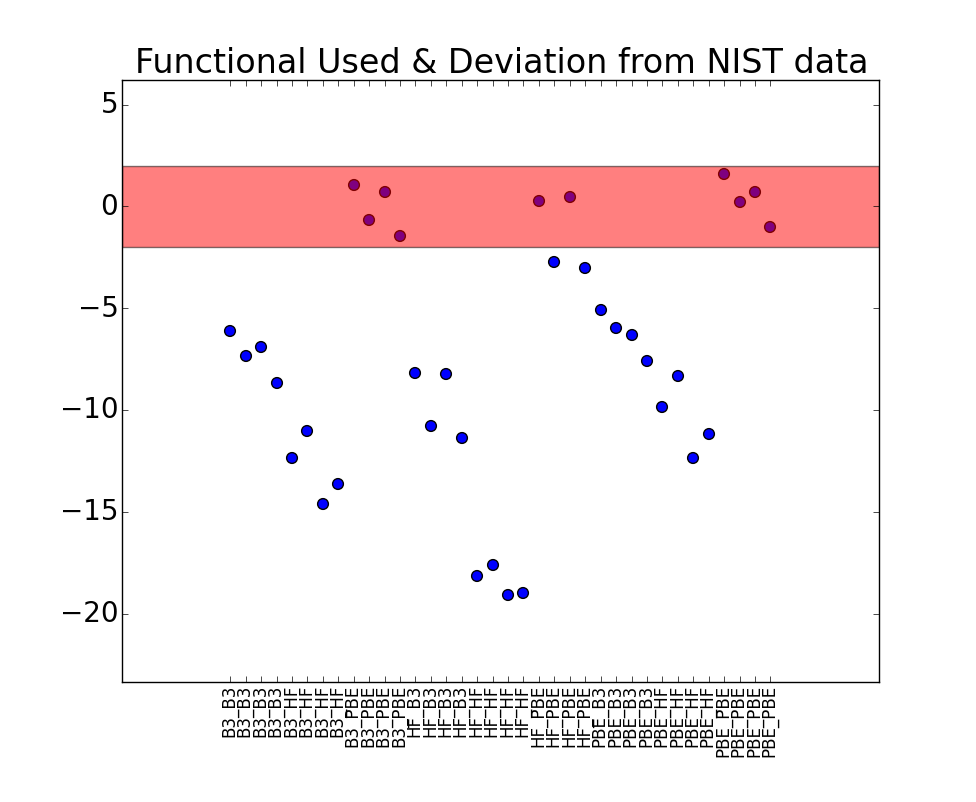
\includegraphics[width=1\textwidth]{Functional_used_Devi_overview.png}
\caption{Overview of Formation Energy Deviation}
\label{fig:overviewdev}
\end{figure} 


\subsection{B3LYP Function and Effect}
If we use B3LYP functional as first stage function, to minimize the deviation from experimental data, we should keep using B3LYP as second stage function from Figure~\ref{fig:B3}. 
\begin{figure}[ht]
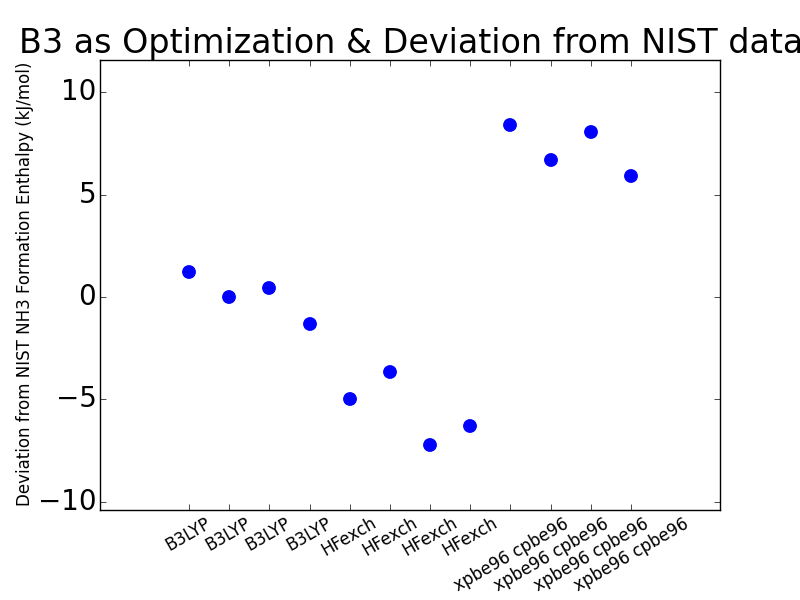
\includegraphics[width=1\textwidth]{B3LYP_Functional_1_Dev.png}
\caption{B3 as geometry optimization stage functional}
\label{fig:B3}
\end{figure} 

\subsection{HF Function and Effect}
If we use HFexch functional as first stage function, to minimize the deviation from experimental data, B3LYP should still be considered as second stage function Figure~\ref{fig:HF}. 
\begin{figure}[ht]
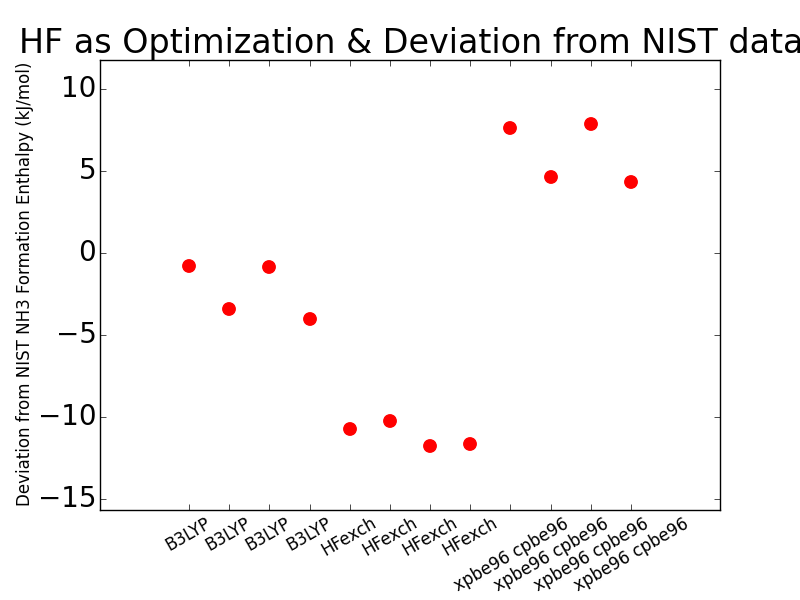
\includegraphics[width=1\textwidth]{HF_Functional_1_Dev.png}
\caption{HF as geometry optimization stage functional}
\label{fig:HF}
\end{figure} 

\subsection{PBE Function and Effect}
If we use PBE functional as first stage function, to minimize the deviation from experimental data, B3LYP should still be considered as second stage function Figure~\ref{fig:PBE}. 
\begin{figure}[ht]
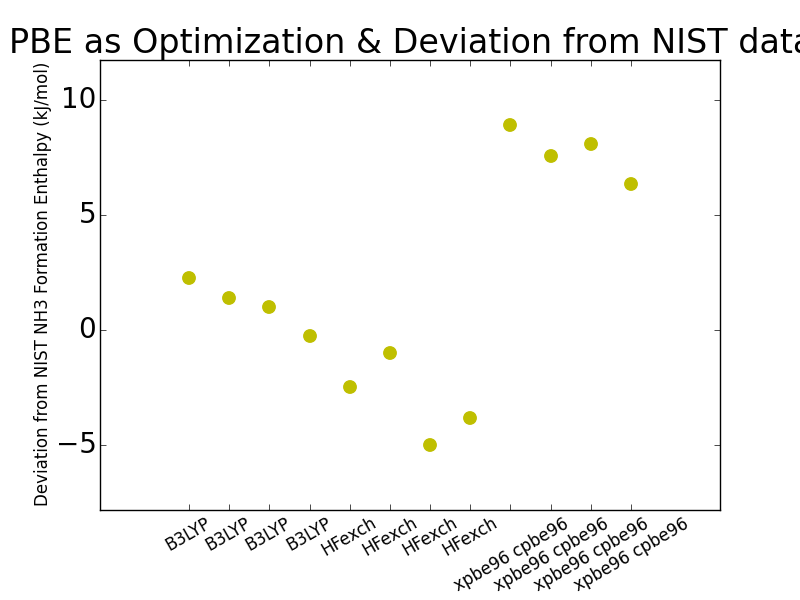
\includegraphics[width=1\textwidth]{PBE_Functional_1_Dev.png}
\caption{PBE as geometry optimization stage functional}
\label{fig:PBE}
\end{figure} 

\subsection{Function and Geometry Angle Prediction}
Using different functional, the N-H bond predicted are not much different and all pretty close to the data we found from online source wiki \cite{Wiki}, as show in Figure~\ref{fig:Geometry}. The blue horizontal line is the experimental angle data we found from wiki. 
\begin{figure}[ht]
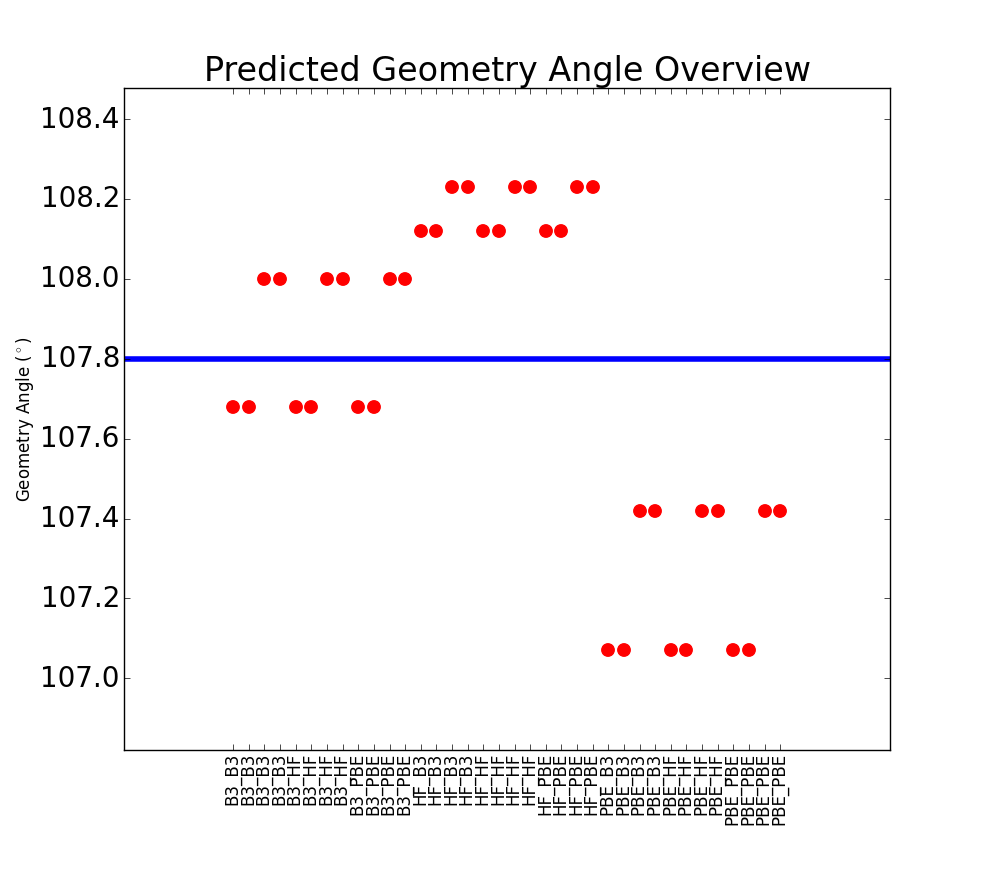
\includegraphics[width=1\textwidth]{Geometry.png}
\caption{N-H angle predicted by various functional set}
\label{fig:Geometry}
\end{figure}

\subsection{Function and Bond Length Prediction}
Using different functional, the N-H bond length predicted are not much different and all pretty close to the data we found from online source wiki \cite{Wiki}, as show in Figure~\ref{fig:Bond Length}. The blue horizontal line is the experimental angle data we found from wiki. The B3LYP functional use 6-31+G* (optimization stage) and 6-311+G* (energy stage) gives the best geometry prediction with highest accuracy.
\begin{figure}[ht]
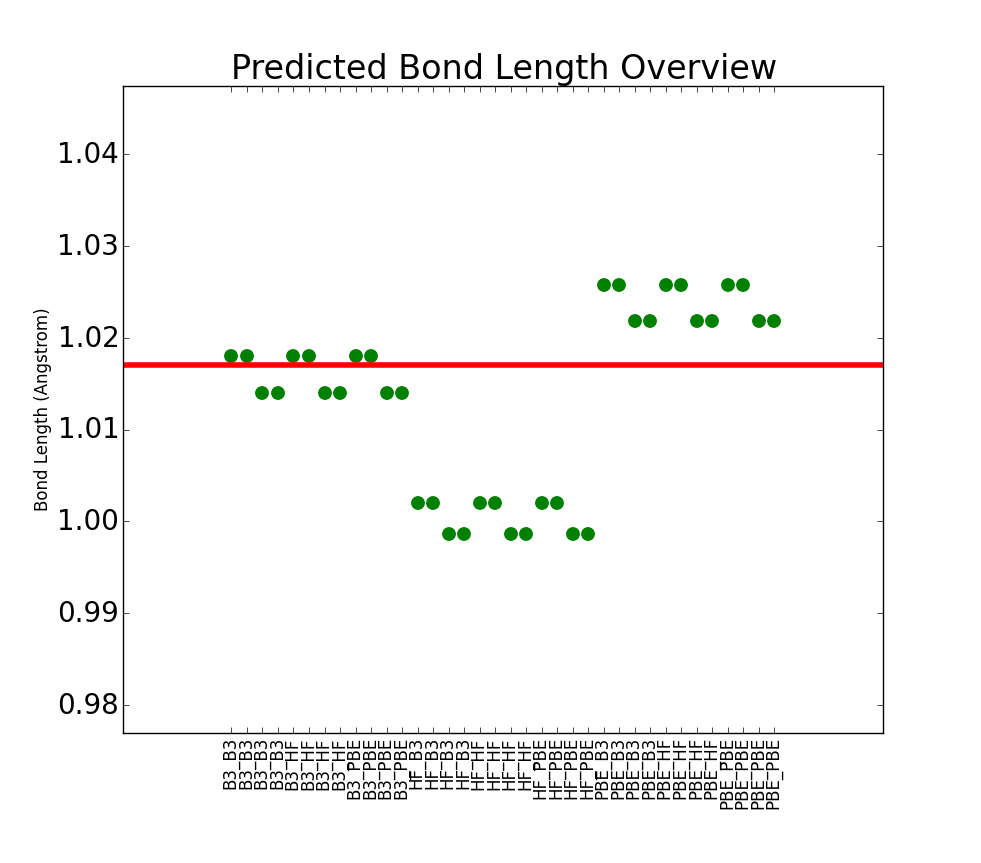
\includegraphics[width=1\textwidth]{Bond_Length.png}
\caption{N-H bond length predicted by various functional set}
\label{fig:Bond Length}
\end{figure}

\subsection{CPU wall time and effectiveness}
If we could accept $2\%$ as deviation, from Figure~\ref{fig:walltime}, using HF functional for geometry optimization and PBE for DFT energy calculation might be the most efficient calculation strategy with relatively good accuracy within 2\%. 
\begin{figure}[ht]
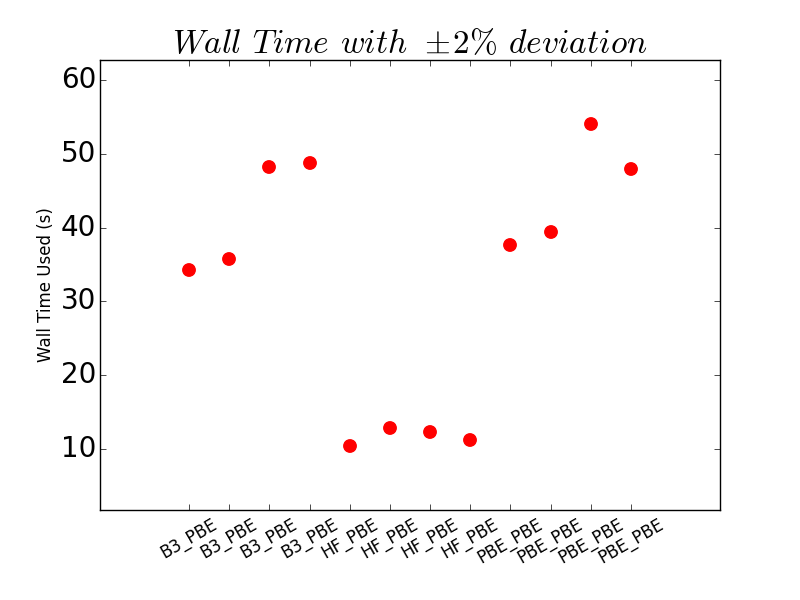
\includegraphics[width=1\textwidth]{walltime.png}
\caption{CPU walltime summary within acceptable deviation}
\label{fig:walltime}
\end{figure}

\subsection{Basis set effect}
In this section, we will investigate the effect of 6-31+G* and 6-311+G* basis set in second stage (DFT energy calculation) calculation, from the below bar chart~\ref{fig:6_31}, using 6-311+G* as second stage function, the predicted formation energy is more close to experimental value with decreased standard deviation also. 

\begin{tabular}{ll}
Row content & Formation Enthalpy(kJ/mol) \\
6-31+G* mean value & -39.640336 \\
6-31+G* standard deviation & 6.651545 \\ 
6-311+G* mean value & -38.815557\\
6-311+G* standard deviation & 5.669244 \\ 
\end{tabular}

\begin{tabular}{llll}
Row content & Wall Time (s) & N-H Angle & N-H Length\\
6-31+G* mean value & 26.588889 & 107.623333 & 1.015263 \\
6-31+G* standard deviation & 13.591214 &   0.456645 & 0.010470\\ 
6-311+G* mean value & 26.588889 & 107.623333 & 1.015263 \\
6-311+G* standard deviation & 13.282392 &  0.456645 & 0.010470\\ 
\end{tabular}

\begin{figure}[ht]
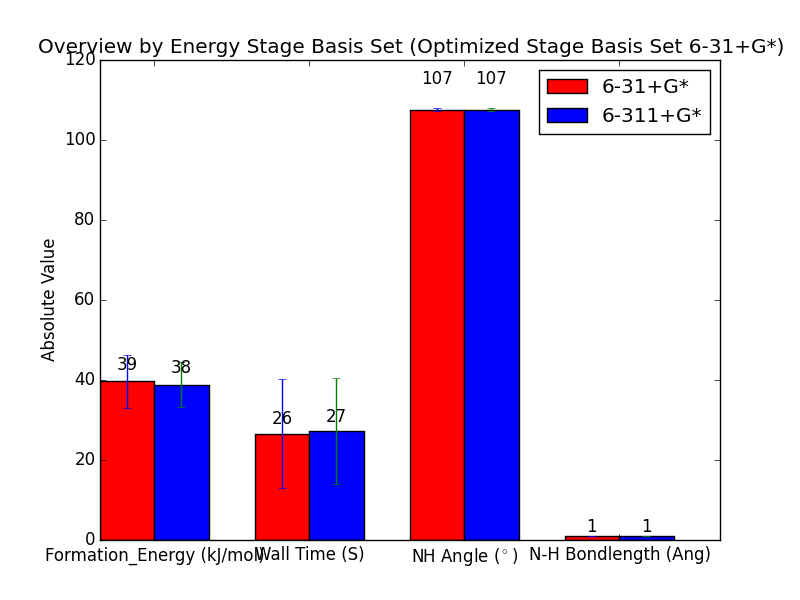
\includegraphics[width=1.2\textwidth]{Basis_Set_6_31_1st.png}
\caption{CPU walltime summary within acceptable deviation}
\label{fig:6_31}
\end{figure}


%----------------------------------------------------------------------------------------
%	SECTION 6
%----------------------------------------------------------------------------------------
\section{Question 6}

For the reaction to happen, we need to break $N-N$ triple bond, the atomic energy of each N is -54.6 Ha. Compared with energy of N2, -109.53 Ha, the dissociation energy of N2 is 0.33 Ha = 8.98 ev, 207.08 kcal/mol. This is also the reaction barrier of reaction. 


%----------------------------------------------------------------------------------------
%	BIBLIOGRAPHY
%----------------------------------------------------------------------------------------

\bibliographystyle{apalike}

\bibliography{sample}

%----------------------------------------------------------------------------------------


\end{document}